\documentclass{scrartcl}
\usepackage[a4paper,top=2cm,bottom=2.5cm,left=2.5cm,right=2.5cm,marginparwidth=0cm]{geometry}
\usepackage[english]{babel}

\usepackage[
    doi=true,
    language=english,
    natbib=true,
    sortcites,
    style=unified,
    useprefix=true,
    ]{biblatex}


% Fonts, languages
\usepackage[warnings-off={mathtools-colon, mathtools-overbracket}]{unicode-math}
\usepackage{fontspec}
\defaultfontfeatures{Ligatures=TeX}
\usepackage[sb]{libertinus-otf}
\usepackage[scale=MatchLowercase]{FiraMono}
\usepackage{fontawesome5}

% Nicer tables
\usepackage{booktabs}
\usepackage[table]{xcolor}
\usepackage{colortbl}
\usepackage[nopatch=footnote]{microtype}
\usepackage{tabularx}

\usepackage[unicode,hidelinks]{hyperref}
\usepackage[normalem]{ulem} % for strikethrough \sout

\usepackage{scrlayer-scrpage}
\newpairofpagestyles{titlepage}{%
    \setkomafont{pageheadfoot}{%
        \small\normalfont 
    }
    \rohead{}
    \lohead{}
}
\pagestyle{scrheadings}
\setkomafont{pagenumber}{\footnotesize}%\sffamily}
\setkomafont{pageheadfoot}%
    {\small\addfontfeature{LetterSpace=10,Numbers=OldStyle}\scshape\sffamily}
\clearpairofpagestyles{}
\cfoot[\pagemark]{\pagemark}
\rohead{\MakeLowercase{\emph{\shorttitle}}}
\lohead{\MakeLowercase{\authorlast}}


% Titlepage
\setkomafont{author}{\large\sffamily}


% Chapter/section headings
\setcounter{secnumdepth}{3}

% Linguistics
\usepackage{langsci-gb4e}
\newcommand{\judgement}[1]{\makebox[0pt][r]{#1}}



\usepackage{cleveref}
\usepackage{enumitem}

%% Line breaks
\widowpenalty=10000
\clubpenalty=10000

% useful 
\usepackage{orcidlink}
\newcommand{\email}[1]{\href{mailto:#1}{#1}}

% copyright notice at end
\usepackage[framemethod=TikZ]{mdframed}
\newenvironment{ccnotice}[1]{%
    \begin{mdframed}[%
        linewidth=0pt,
        leftmargin=1pt,
        rightmargin=1pt,
        backgroundcolor=gray!10!white,
        font=\sffamily,
    ]\relax%
}{\end{mdframed}}


\usepackage[autostyle=true,english=american]{csquotes}
\renewcommand*{\mkccitation}[1]{ (#1)}

\usepackage{xcolor}
\usepackage{titlesec}
\definecolor{mycolor}{HTML}{6baefa}
\titleformat{\section}
              {\normalfont\Large\bfseries\color{mycolor}} % Formatting
              {\thesection}            % Label
              {2em}                   % Space after label
              {}  


% title page
\title{\fulltitle}
\date{}



\newcommand{\fulltitle}{Primo Deriverable}

\author{%
    Berardo Cristiano, mat. 234428\\
    De Piccoli Martina, mat.  235165\\
    Vettore Giacomo, mat. XXXXXX
}

\usepackage[linguistics]{forest}

\hypersetup{
    colorlinks=false,
    linkcolor=blue,
    filecolor=magenta,      
    urlcolor=cyan,
    pdftitle={Primo-deliverable-id3},
    pdfpagemode=FullScreen,
    }

\begin{document}

\maketitle
\thispagestyle{titlepage}
\pagestyle{scrheadings}

\begin{abstract}
    \noindent\textbf{Idea di progetto:} \\
\end{abstract}

\newpage
\section{Attori del sistema}
\vspace{-8mm}
\begin{figure}[!h]
    \centering
    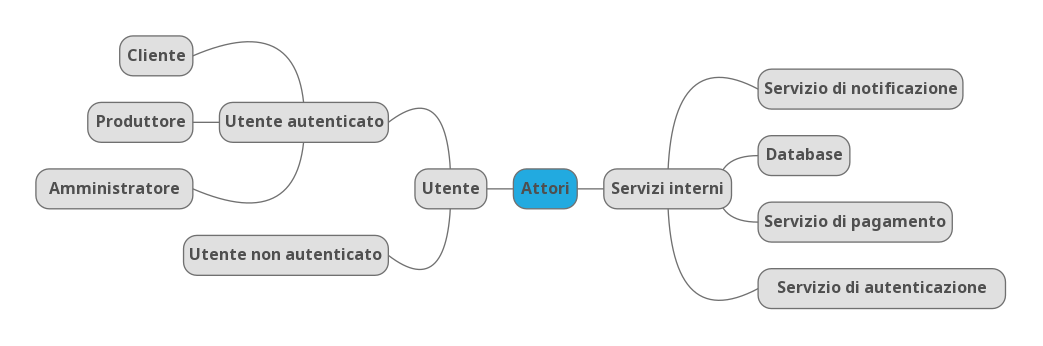
\includegraphics[width=1\linewidth]{Deliverables/first-deliverable/img/mappa_attori.png}
    \label{fig:mindmap}
\end{figure}

\vspace{-10mm}

\begin{attori}
    \itemc
    \end{enumerate}
\end{attori}

\newpage
\section{Requisiti Funzionali}
\noindent

\textbf{RF1}: <id> the system has to <function>

\textbf{RF2}: <id> the system has to <function>
\section{Requisiti non funzionali}

\begin{rnfenum}
    \item \textbf{Sicurezza}:
        
        \begin{rnfenum}
            \item Il sistema deve poter fornire accesso all'area privata di ogni singolo utente grazie a provider OAuth.
            \item Il sistema deve poter fornire accesso all'area privata di ogni singolo utente grazie a mail e password.
            \item Il sistema deve garantire la riservatezza delle password attraverso l'implementazione di meccanismi di sicurezza conformi alle migliori pratiche di settore e allo Stato dell'Arte tecnologico.
            \item Il sistema si dovrà appoggiare a provider esterni per garantire la sicurezza delle transazioni di denaro elettroniche.
        \end{rnfenum}
    
    \item \textbf{Prestazioni}: 

        \begin{rnfenum}
            \item Il sistema deve poter creare un report \textbf{RFXXX}, da quando la richiesta arriva al server, in meno di 3s.
            \item Il sistema deve essere in grado di rispondere entro massimo 3s a tutte le interazioni utente-sistema.
            \item Il sistema deve poter essere monitorato in qualsiasi momento, questo per verificare lo stato di tutto l'applicativo.
        \end{rnfenum}
    
    \item \textbf{Scalabilità}: 
        \begin{rnfenum}
            \item Il sistema deve essere in grado di poter scalare autonomamente in base al carico utente grazie a tecnologie quali Kubernetes e Container.
            \item Il sistema deve essere in grado di poter anche 100 richeste assieme senza perdere prestazione, come descritto da \textbf{RNF2.2}
        \end{rnfenum}

    \item \textbf{Affidabilità}:
        \begin{rnfenum}
            \item Il sistema deve essere avere un uptime del 99.9\%.
        \end{rnfenum}

    \item \textbf{Compatibilità}:
        \begin{rnfenum}
            \item Il sistema deve essere compatibile con i principali browser web Chrome, Firefox e Safari
            \item Il sistema deve essere reso disponibile per tutte le piattaforme: desktop, tablet e mobile
        \end{rnfenum}       

    \item \textbf{Normative}:
        \begin{rnfenum}
            \item Il sistema deve cancellare tutti i dati dell'utente in base alla normativa vigente italiana e secondo le leggi che regolano la privacy, GDPR.
        \end{rnfenum}

    \item \textbf{Sviluppo software}:
        \begin{rnfenum}
            \item Il sistema verrà implementato utilizzando TypeScript, il controllo sui tipi lo rende più immune ad errori umani.
            \item L'integrazione con la repository GitHub necessaria per mantenere lo storico e creare nuove features in parallelo e senza creare danni all'applicazione principale.
            \item Utilizzo di database documentale, MongoDB, per mantenere salvati i dati principali dell' applicazione.
            \item Utilizzo del database Firebase per garantire la possibilità di accesso con GoogleOAuth.
        \end{rnfenum}
    
    
\end{rnfenum}

\newpage
I requisiti non funzionali definiscono \textbf{COME} il sistema deve operare, specificando attributi di qualità e vincoli di sistema.\\
Caratteristiche:

\begin{itemize}
    \item Descrivono qualità e vincoli del sistema
    \item Spesso misurabili su una scala (velocità, affidabilità, ecc.)
    \item Impattano l'architettura e il design del sistema
\end{itemize}

Esempi di requisiti non funzionali:

\begin{enumerate}
    \item Prestazioni: Il sistema deve rispondere alle richieste entro 2 secondi
    \item Sicurezza: Le password devono essere criptate con algoritmo SHA-256
    \item Usabilità: L'interfaccia deve essere accessibile secondo standard WCAG 2.1
    \item Scalabilità: Il sistema deve supportare fino a 10.000 utenti concorrenti
    \item Affidabilità: Il sistema deve avere un uptime del 99,9%
    \item Manutenibilità: Il codice deve seguire standard di codifica specifici
    \item Compatibilità: L'applicazione deve funzionare sui browser Chrome, Firefox e Safari
\end{enumerate}

Differenze Principali

Focus:

\begin{itemize}
    \item Funzionali: cosa fa il sistema
    \item Non funzionali: come lo fa e quanto bene lo fa
\end{itemize}


Misurazione:

\begin{itemize}
    \item Funzionali: binaria (soddisfatto o non soddisfatto)
    \item Non funzionali: continua (livelli di prestazione)
\end{itemize}


Impatto sul design:

\begin{itemize}
    \item Funzionali: influenzano principalmente le funzionalità specifiche
    \item Non funzionali: influenzano l'intera architettura del sistema
\end{itemize}


Priorità:

\begin{itemize}
    \item Funzionali: facilmente prioritizzabili dai clienti
    \item Non funzionali: spesso determinati da considerazioni tecniche
\end{itemize}
\section{Use-cases}



\end{document}
